%<<echo=FALSE>>=
%OLD <- options(width=90)
%@
%<<echo=FALSE>>=
%options(OLD) 
%@

\documentclass{beamer}\usepackage[]{graphicx}\usepackage[]{color}
%% maxwidth is the original width if it is less than linewidth
%% otherwise use linewidth (to make sure the graphics do not exceed the margin)
\makeatletter
\def\maxwidth{ %
  \ifdim\Gin@nat@width>\linewidth
    \linewidth
  \else
    \Gin@nat@width
  \fi
}
\makeatother

\definecolor{fgcolor}{rgb}{0.102, 0.102, 0.102}
\newcommand{\hlnum}[1]{\textcolor[rgb]{0.2,0.2,0.2}{#1}}%
\newcommand{\hlstr}[1]{\textcolor[rgb]{0.2,0.2,0.2}{#1}}%
\newcommand{\hlcom}[1]{\textcolor[rgb]{0.302,0.302,0.302}{\textit{#1}}}%
\newcommand{\hlopt}[1]{\textcolor[rgb]{0.102,0.102,0.102}{#1}}%
\newcommand{\hlstd}[1]{\textcolor[rgb]{0.102,0.102,0.102}{#1}}%
\newcommand{\hlkwa}[1]{\textcolor[rgb]{0.102,0.102,0.102}{#1}}%
\newcommand{\hlkwb}[1]{\textcolor[rgb]{0.102,0.102,0.102}{#1}}%
\newcommand{\hlkwc}[1]{\textcolor[rgb]{0.2,0.2,0.2}{#1}}%
\newcommand{\hlkwd}[1]{\textcolor[rgb]{0.102,0.102,0.102}{\textbf{#1}}}%

\usepackage{framed}
\makeatletter
\newenvironment{kframe}{%
 \def\at@end@of@kframe{}%
 \ifinner\ifhmode%
  \def\at@end@of@kframe{\end{minipage}}%
  \begin{minipage}{\columnwidth}%
 \fi\fi%
 \def\FrameCommand##1{\hskip\@totalleftmargin \hskip-\fboxsep
 \colorbox{shadecolor}{##1}\hskip-\fboxsep
     % There is no \\@totalrightmargin, so:
     \hskip-\linewidth \hskip-\@totalleftmargin \hskip\columnwidth}%
 \MakeFramed {\advance\hsize-\width
   \@totalleftmargin\z@ \linewidth\hsize
   \@setminipage}}%
 {\par\unskip\endMakeFramed%
 \at@end@of@kframe}
\makeatother

\definecolor{shadecolor}{rgb}{.97, .97, .97}
\definecolor{messagecolor}{rgb}{0, 0, 0}
\definecolor{warningcolor}{rgb}{1, 0, 1}
\definecolor{errorcolor}{rgb}{1, 0, 0}
\newenvironment{knitrout}{}{} % an empty environment to be redefined in TeX

\usepackage{alltt}% regular slides (with pauses)
%\documentclass[handout]{beamer}% handout (no pauses)

%%%%%%%%%%%%%%%%%%%%%%%%%%%%%%%%%%%%%%%%%%%%%%%%%%%%%%%%%%%%%%%%%%%%%%%%%
%%%%%%% Change the lecture information here %%%%%%%%%%%%%%%%
\def\chapnum{Week \#5}
\title{STAT234: Lecture 7 - Type I, Type II and Power}
\author{Kushal K. Dey}
\date{}
%%%%%%%%%%%%%%%%%%%%%%%%%%%%%%%%%%%%%%%%%%%%%%%%%%%%%%%%%%%%%%%%%%%%%%%%%

%%%%%% Start of suggested definitions and packages %%%%%%%%%%%%
%%%%%% Do not change unless you really know what you are doing %%%%%%%%%%
%%%%%%%%%%%%%%%%%%%%%%%%%%%%%%%%%%%%%%%%%%%%%%%%%%%%%%%%%%%%%%%%%%%%%%%%%

\usepackage{enumerate}
\usepackage{amsmath, bbm}
\usepackage[misc]{ifsym} % for the dice symbol \Cube{}
\usepackage[latin1]{inputenc}
\usepackage{hyperref}
\usepackage{multirow}

%\usepackage{comment}
%\usepackage{pstricks}
%\usepackage{graphicx}
%\usepackage{booktabs}
%\usepackage{pgfpages}
%\pgfpagesuselayout{2 on 1}[a4paper,border shrink=3mm]
%\pgfpagesuselayout{4 on 1}[a4paper,landscape,border shrink=3mm

\usepackage{setspace}
\ifdefined\knitrout
  \renewenvironment{knitrout}{\begin{spacing}{0.75}\begin{tiny}}{\end{tiny}\end{spacing}}
\else
\fi

%%%%%%%%%%%%%%% Defined Shortcuts (macros) %%%%%%%%%%%%%
% parameters and statistics
\newcommand{\xbar}{\overline{x}}
\newcommand{\Xbar}{\overline{X}}
\newcommand{\ybar}{\overline{y}}
\newcommand{\Ybar}{\overline{Y}}
\newcommand{\dbar}{\overline{d}}
\newcommand{\Dbar}{\overline{D}}
\newcommand{\zbar}{\overline{z}}
\newcommand{\Zbar}{\overline{Z}}
\newcommand{\ehat}{\widehat{\epsilon}}
\newcommand{\yhat}{\widehat{y}}
\newcommand{\Yhat}{\widehat{Y}}
\newcommand{\betaa}{{\beta_0}}
\newcommand{\betab}{{\beta_1}}
\newcommand{\betac}{{\beta_2}}
\newcommand{\betad}{{\beta_3}}
\newcommand{\BETA}{{\boldsymbol\beta}}
\newcommand{\betahata}{\widehat{\beta_0}}
\newcommand{\betahatb}{\widehat{\beta_1}}
\newcommand{\betahatc}{\widehat{\beta_2}}
\newcommand{\betahatd}{\widehat{\beta_3}}
\newcommand{\bhat}{\widehat{b}}
\newcommand{\btilde}{\widetilde{b}}
\newcommand{\ahat}{\widehat{a}}
\newcommand{\atilde}{\widetilde{a}}
\newcommand{\rss}{\mathit{SSE}}
\newcommand{\sigmahat}{\widehat{\sigma}}
\newcommand{\betahat}{\widehat{\beta}}
\newcommand{\thetahat}{\widehat{\theta}}
\newcommand{\phat}{\widehat{p}}
\newcommand{\pihat}{\widehat{\pi}}
\newcommand{\muhat}{\widehat{\mu}}
% real numbers and integers
\newcommand{\reals}{\mathbbm{R}}
\newcommand{\integers}{\mathbbm{N}}
%distributions
\newcommand{\normal}{\textsf{Norm}}
\newcommand{\Bin}{\textsf{Binom}}
\newcommand{\Uni}{\textsf{Unif}}
\newcommand{\Poisson}{\textsf{Pois}}
\newcommand{\Exp}{\textsf{Exp}}
\newcommand{\Beta}{\textsf{Beta}}
\newcommand{\iid}{\stackrel{\mathrm{iid}}{\sim}}
% probability and expected value
\newcommand{\rv}{r.v.\ }
\newcommand{\prob}{{\rm P}}
\newcommand{\mean}{\mathrm{E}}
\newcommand{\var}{\mathrm{Var}}
\newcommand{\Var}{\mathrm{Var}}
\newcommand{\cov}{\mathrm{Cov}}
\newcommand{\corr}{\mathop{\mathrm{Corr}}}
% measures of spread
\newcommand{\IQR}{\textit{IQR}}
\newcommand{\SAD}{\textit{SAD}}
\newcommand{\MAD}{\textit{MAD}}
\newcommand{\SSD}{\textit{SSD}}
\newcommand{\MSD}{\textit{MSD}}
\newcommand{\RMSD}{\textit{RMSD}}
\newcommand{\MSE}{\textit{MSE}}
\newcommand{\MSR}{\textit{MSR}}
% formatting code and such
\providecommand{\variable}[1]{}
\renewcommand{\variable}[1]{{\color{green!50!black}\texttt{#1}}}
\providecommand{\function}[1]{}
\renewcommand{\function}[1]{{\color{purple!75!blue}\texttt{\StrSubstitute{#1}{()}{}()}}}
\providecommand{\option}[1]{}
\renewcommand{\option}[1]{{\color{brown!80!black}\texttt{#1}}}
\providecommand{\pkg}[1]{}
\renewcommand{\pkg}[1]{{\color{red!80!black}\texttt{#1}}}
\providecommand{\code}[1]{}
\renewcommand{\code}[1]{{\color{blue!80!black}\texttt{#1}}}

%%%%%%%%%
% Changed by Kushal K Dey, University of Chicago
%\providecommand{\file}[1]{}
%\renewcommand{\file}[1]{{\tt #1}}
\providecommand{\file}[1]{}
\renewcommand{\file}[1]{{\color{orange!80!black}\texttt{#1}}}
%\providecommand{\dataframe}[1]{}
%\renewcommand{\dataframe}[1]{{\color{blue!80!black}\texttt{#1}}}
\providecommand{\dataframe}[1]{}
\renewcommand{\dataframe}[1]{{\color{cyan!80!black}\texttt{#1}}}
%%%%%%%%%

% other
\def\Sum{\sum\nolimits}
\def\b#1{\fboxsep=0pt\colorbox{black}{\color{white}\Cube{#1}}}
\def\w#1{\Cube{#1}}
%%%%%%%%%%%% End of shortcuts (macros) ##############

%%%%%%%%% One way to hide answers until you want to show them %%%%%%%%%
\def\Hide#1#2{\ul{~~~\onslide<#1>{\alert{#2}}~~~}}
\def\hide#1#2{\ul{~~\onslide<#1>{\alert{#2}}~~}}
\def\hid#1#2{\onslide<#1>{\alert{#2}}}
% Choose the color of answers here too
\setbeamercolor{alerted text}{fg=darkgray} 
%\setbeamercolor{alerted text}{fg=black} 

%------Centered Page Number Setup ------
\defbeamertemplate{footline}{centered page number}
{%
  \hspace*{\fill}%
  %\usebeamercolor[fg]{page number in head/foot}%
  %\usebeamerfont{page number in head/foot}%
  \tiny \chapnum: Page \insertframenumber\, of \inserttotalframenumber%
  \hspace*{\fill}\vskip2pt%
}
%\setbeamertemplate{footline}{\hfill\insertframenumber/\inserttotalframenumber}
\setbeamertemplate{footline}[centered page number]
%--------------------------------

%\usetheme{Copenhagen}
\setbeamertemplate{navigation symbols}{}
\usepackage[english]{babel}
\def\ul{\underline}
\linespread{1.1}
% or whatever



%\parskip=0pt
\IfFileExists{upquote.sty}{\usepackage{upquote}}{}
\begin{document}%large

%<<setup, include=FALSE, cache=FALSE>>=
%options(replace.assign=TRUE,width=90, digits=4)
%opts_chunk$set(fig.path='figure/graphics-', cache.path='cache/graphics-', fig.align='center', fig.width=8, fig.height=4.5, fig.show='as.is', out.width='0.9\\linewidth', cache=FALSE, par=TRUE, size = 'tiny', tidy=TRUE, cache.extra=rand_seed)
%knit_hooks$set(par=function(before, options, envir){
%if (before && options$fig.show!='none') par(mar=c(4,4,.1,.1),cex.lab=.95,cex.axis=.9,mgp=c(2,.7,0),tcl=-.3)
%}, document = function(x) {
%  gsub('\\\\(begin|end)\\{kframe\\}', '', x)
%}, crop=hook_pdfcrop)
%@
%<<setup2, include=FALSE, cache=FALSE>>=
%knit_theme$set("print")
%@


%%%%%%%%%%%%%%%%%%%%%%%%%%%%%%%%%%%%%%%%%%%%%%%%%%%%%%%%%%%%%%%%%%%%%%%%%
%%%%%%%%%%%%%%%%%%%%%%%%%%%%%%%%%%%%%%%%%%%%%%%%%%%%%%%%%%%%%%%%%%%%%%%%%
%%%%%% End of suggested definitions and packages %%%%%%%%%%%%

%------------------------------------------------------------------
%------------------------------------------------------------------

%%%%%%%%%% Title frame (optional) %%%%%%%%%%%%%
\begin{frame}{}
\maketitle
\end{frame}
%%%%%%%%%%%%%%%%%%%%%%%%%%%%%%%%%%%%%%%%%%%%%%%

%%%%%%%%%%%%%% Begin slides here %%%%%%%%%%%%%%

%%%%%%%%%%%%%%%%%%%%%%%%%%%%%%%%%%%%%%%%%%%%%%%
\begin{frame}
%%%%%%%%%%%%%%%%%%%%%%%%%%%%%%%%%%%%%%%%%%%%%%%

Last class \pause \newline

\begin{itemize}
\item Type I error : Probability that we reject the null hypothesis when it is true (fair for statistician) \pause

\item Type II error: Probability that we accept the null hypothesis when it is false (fair for the researcher) \pause

\item Power: 

$$  Power = 1 - Type \; II \; error $$

It is the probability that we reject the null hypothesis when it is false. \pause \newline

\textit{We want to minimize Type I error and maximize Power}

\end{itemize}
\end{frame}
%%%%%%%%%%%%%%%%%%%%%%%%%%%%%%%%%%%%%%%%%%%%%%%


%%%%%%%%%%%%%%%%%%%%%%%%%%%%%%%%%%%%%%%%%%%%%%%
\begin{frame}{Two Types of Errors Revisited}
%%%%%%%%%%%%%%%%%%%%%%%%%%%%%%%%%%%%%%%%%%%%%%%

%  \begin{small}
    Recall that the following four outcomes are possible when conducting
    a test:

    \begin{center}
      \begin{tabular}{|c|c|c|}
        \hline
        \multirow{2}{*}{Reality} & \multicolumn{2}{c|}{Our Decision}\\
        & \multicolumn{1}{c}{$H_0$} & $H_a$\\
        \hline
        \multirow{2}{*}{$H_0$} & $\surd$ & Type I Error\\
        & ($\mbox{Prob}=1-\alpha$) & ($\mbox{Prob}=\alpha$)\\
        \cline{2-3}
        \multirow{2}{*}{$H_a$} & Type II Error & $\surd$\\
        & ($\mbox{Prob}=\beta$) & ($\mbox{Prob}=1-\beta$)\\
        \hline
      \end{tabular}
    \end{center}
\pause
    Type I error is generally {\bf more serious} than type II error. \\ \pause
    For example: $H_0:$ the person is not guilty, $H_1:$ the person is guilty\\ \pause
    Type I error \pause = convicting an innocent person\\ \pause
    Type II error \pause = failing to convict a guilty person\\ \pause
    In practice, we first choose an $\alpha$ and consider only tests
    with probability of Type I error no greater than $\alpha$. \pause Then we select one that makes Type II error as small as possible (test with most power). \pause
%  \end{small}

\end{frame}
%%%%%%%%%%%%%%%%%%%%%%%%%%%%%%%%%%%%%%%%%%%%%%%

%%%%%%%%%%%%%%%%%%%%%%%%%%%%%%%%%%%%%%%%%%%%%%%
\begin{frame}{Hypothesis testing framework}
%%%%%%%%%%%%%%%%%%%%%%%%%%%%%%%%%%%%%%%%%%%%%%%

Last time we considered the example, 

$X_1, X_2, \cdots, X_{n}$ be data coming from 

$$ X_{i} \sim N(\mu, \sigma^2) $$ 

and we assumed that we know $\sigma^2$. In our model, 

$$ \sigma = 2 $$ 

Hypothesis to test 

$$ H_0: \mu=0 \;\; H_1: \mu > 0 $$ 

We want to choose smallest $c$ such that $\bar{X} > c$ happens with probability  greater than or equal to the Type I error ($0.05$)

$$ find \; smallest \; c\; : Pr \left [ \bar{X} > c | \mu=0 \right] < 0.05 $$

\end{frame}
%%%%%%%%%%%%%%%%%%%%%%%%%%%%%%%%%%%%%%%%%%%%%%%

%%%%%%%%%%%%%%%%%%%%%%%%%%%%%%%%%%%%%%%%%%%%%%%
\begin{frame}{Hypothesis testing framework}
%%%%%%%%%%%%%%%%%%%%%%%%%%%%%%%%%%%%%%%%%%%%%%%

$$ Type \; I \; error: Pr \left [ Z > \frac{\sqrt{n}}{\sigma}c | \mu=0 \right ] = 0.05  \hspace{1 cm} Z \sim N(0,1) $$ 

From this, we know 

$$ \frac{\sqrt{n}}{\sigma}c = 1.644  $$ 

Our case: $\sigma=2$ and $n=25$ resulted in $c=0.658$. 
Power needs a $\mu$ under alternate hypothesis. If we assume $\mu=1$,

$$ Power: Pr \left [ \bar{X} > 0.658 | \mu=1 \right] $$

$$ Power(1):  Pr \left [ Z > \frac{\sqrt{n}}{\sigma}(c-1)  \right] \; Z \sim N(0,1) $$

\end{frame}
%%%%%%%%%%%%%%%%%%%%%%%%%%%%%%%%%%%%%%%%%%%%%%%

%%%%%%%%%%%%%%%%%%%%%%%%%%%%%%%%%%%%%%%%%%%%%%%
\begin{frame}{Hypothesis testing framework}
%%%%%%%%%%%%%%%%%%%%%%%%%%%%%%%%%%%%%%%%%%%%%%%

The right hand side quantity 

$$ \frac{\sqrt{n}}{\sigma}(c-1) = \frac{\sqrt{n}}{\sigma}c - \frac{\sqrt{n}}{\sigma} $$ \pause

here at $5\%$ level of significance,

$$ \frac{\sqrt{n}}{\sigma}(c-1) = 1.644 - \frac{\sqrt{n}}{\sigma} $$

$$ Power:  Pr \left [ Z > 1.644 - \frac{\sqrt{n}}{\sigma}  \right] \; Z \sim N(0,1) $$ \pause

As $\sigma$ decreases or $n$ increases, we have higher power. \pause 

But we do not control $\sigma$, we can only control $n$. \pause

\end{frame}
%%%%%%%%%%%%%%%%%%%%%%%%%%%%%%%%%%%%%%%%%%%%%%%

%%%%%%%%%%%%%%%%%%%%%%%%%%%%%%%%%%%%%%%%%%%%%%%
\begin{frame}{Hypothesis testing framework}
%%%%%%%%%%%%%%%%%%%%%%%%%%%%%%%%%%%%%%%%%%%%%%%

Suppose I say I want my power to be $0.99$ at $5\%$ level of siginifance. \pause

We know that 

$$ Type \; I \; error: Pr \left [ Z > \frac{\sqrt{n}}{\sigma}c | \mu=0 \right ] = 0.05  \hspace{1 cm} Z \sim N(0,1) $$  \pause

From this, we know 

$$ \frac{\sqrt{n}}{\sigma}c = 1.644  $$  \pause

and 

$$ Power:  Pr \left [ Z > 1.644 - \frac{\sqrt{n}}{\sigma}  \right] \; Z \sim N(0,1) $$

\end{frame}
%%%%%%%%%%%%%%%%%%%%%%%%%%%%%%%%%%%%%%%%%%%%%%%

%%%%%%%%%%%%%%%%%%%%%%%%%%%%%%%%%%%%%%%%%%%%%%%
\begin{frame}{Hypothesis testing framework}
%%%%%%%%%%%%%%%%%%%%%%%%%%%%%%%%%%%%%%%%%%%%%%%

$$ 1.644 - \frac{\sqrt{n}}{2} =  -2.32 $$ \pause

$$ \sqrt{n} = 2*(2.32+1.644)= 7.928 $$ \pause

$$ n \approx 65$$ \pause

So just collecting $65$ samples under this testing framework we have can give us a Power of $0.99$ at $\mu=1$ or Type II error as low as $0.01$ given that we fix the Type I error to be $0.05$. \pause

So, we can decide on how many samples to choose by deciding on the Type I and Type II errors we want.

\end{frame}
%%%%%%%%%%%%%%%%%%%%%%%%%%%%%%%%%%%%%%%%%%%%%%%


%%%%%%%%%%%%%%%%%%%%%%%%%%%%%%%%%%%%%%%%%%%%%%%
\begin{frame}{Hypothesis testing framework}
%%%%%%%%%%%%%%%%%%%%%%%%%%%%%%%%%%%%%%%%%%%%%%%

But $\mu=1$ is only one possible alternative for the hypothesis. So, what we would want to do is get a formula of power for each value of $\mu$ in the alternate space.

$$ Power(\mu):  Pr \left [ Z > \frac{\sqrt{n}}{\sigma}(c-\mu)  \right] \; Z \sim N(0,1) $$

Since from Type I error argument, we showed that 

$$ \frac{\sqrt{n}}{\sigma}c = 1.644 $$

$$ Power(\mu):  Pr \left [ Z > 1.644 - \frac{\sqrt{n}}{\sigma}\mu  \right] \; Z \sim N(0,1) $$

This can be written as 

$$ Power(\mu): = \Phi \left (\frac{\sqrt{n}}{\sigma}\mu - 0.644 \right) $$

\end{frame}
%%%%%%%%%%%%%%%%%%%%%%%%%%%%%%%%%%%%%%%%%%%%%%%

%%%%%%%%%%%%%%%%%%%%%%%%%%%%%%%%%%%%%%%%%%%%%%%
\begin{frame}{Hypothesis testing framework}
%%%%%%%%%%%%%%%%%%%%%%%%%%%%%%%%%%%%%%%%%%%%%%%

We plot $Power(\mu)$ against $\mu$.  Say $n=65$ and we know $\sigma=2$. \newline

\begin{knitrout}\small
\definecolor{shadecolor}{rgb}{1, 1, 1}\color{fgcolor}

{\centering \includegraphics[width=0.99\linewidth]{figure/graphics-unnamed-chunk-1-1} 

}



\end{knitrout}

\end{frame}
%%%%%%%%%%%%%%%%%%%%%%%%%%%%%%%%%%%%%%%%%%%%%%%

%%%%%%%%%%%%%%%%%%%%%%%%%%%%%%%%%%%%%%%%%%%%%%%
\begin{frame}{Hypothesis testing framework}
%%%%%%%%%%%%%%%%%%%%%%%%%%%%%%%%%%%%%%%%%%%%%%%

We plot $Power(\mu)$ against $\mu$.  Say $n=25$ and we know $\sigma=2$. \newline

\begin{knitrout}\small
\definecolor{shadecolor}{rgb}{1, 1, 1}\color{fgcolor}

{\centering \includegraphics[width=0.99\linewidth]{figure/graphics-unnamed-chunk-2-1} 

}



\end{knitrout}

\end{frame}
%%%%%%%%%%%%%%%%%%%%%%%%%%%%%%%%%%%%%%%%%%%%%%%

%%%%%%%%%%%%%%%%%%%%%%%%%%%%%%%%%%%%%%%%%%%%%%%
\begin{frame}{Hypothesis testing framework}
%%%%%%%%%%%%%%%%%%%%%%%%%%%%%%%%%%%%%%%%%%%%%%%

We plot $Power(\mu)$ against $\mu$.  Say $n=25$ and we know $\sigma=0.1$. \newline

\begin{knitrout}\small
\definecolor{shadecolor}{rgb}{1, 1, 1}\color{fgcolor}

{\centering \includegraphics[width=0.99\linewidth]{figure/graphics-unnamed-chunk-3-1} 

}



\end{knitrout}

\end{frame}
%%%%%%%%%%%%%%%%%%%%%%%%%%%%%%%%%%%%%%%%%%%%%%%

%%%%%%%%%%%%%%%%%%%%%%%%%%%%%%%%%%%%%%%%%%%%%%%
\begin{frame}{Hypothesis testing framework}
%%%%%%%%%%%%%%%%%%%%%%%%%%%%%%%%%%%%%%%%%%%%%%%

\begin{itemize}

\item As $\sigma$ decreases (for fixed $n$), the power curve becomes steeper and reaches $1$ early (Type II error decreases steeply to $0$). \pause \newline

\item As $n$ increases (for fixed $\sigma$), the power curve becomes steeper and reaches $1$ early. As $n$ decreases, the power curve takes more time to reach $1$. \pause \newline

\item for fixed $\sigma$, the power for higher $n$ remains higher at each $\mu$. For fixed $n$, the power for lower $\sigma$ remains higher at each $\mu$

\end{itemize}

\end{frame}
%%%%%%%%%%%%%%%%%%%%%%%%%%%%%%%%%%%%%%%%%%%%%%%


%%%%%%%%%%%%%%%%%%%%%%%%%%%%%%%%%%%%%%%%%%%%%%%
\begin{frame}
%%%%%%%%%%%%%%%%%%%%%%%%%%%%%%%%%%%%%%%%%%%%%%%

\begin{center}
\huge{Another important continuous distribution }
\end{center}
\end{frame}
%%%%%%%%%%%%%%%%%%%%%%%%%%%%%%%%%%%%%%%%%%%%%%%

%%%%%%%%%%%%%%%%%%%%%%%%%%%%%%%%%%%%%%%%%%%%%%%
\begin{frame}{Chi-Square Distribution}
%%%%%%%%%%%%%%%%%%%%%%%%%%%%%%%%%%%%%%%%%%%%%%%

The chi-square distributions: $\chi_k^2$
$$f(x) = \frac{ x^{(k/2)-1} e^{- x/2}}{2^{k/2}\Gamma(k/2)}
  \qquad x>0,\, k\geq 1$$ \pause
$$E(X) = k \qquad Var(X) = 2k$$ \pause

\begin{center}
\includegraphics[width=8cm,height=4cm]{chi-square}
\end{center}


\end{frame}
%%%%%%%%%%%%%%%%%%%%%%%%%%%%%%%%%%%%%%%%%%%%%%%

%%%%%%%%%%%%%%%%%%%%%%%%%%%%%%%%%%%%%%%%%%%%%%%
\begin{frame}{Chi-Square Distribution}
%%%%%%%%%%%%%%%%%%%%%%%%%%%%%%%%%%%%%%%%%%%%%%%

The chi-square distributions: $\chi_1^2$
$$f(x) = \frac{ x^{-1/2} e^{- x/2}}{\sqrt{2\pi}}
  \qquad x>0$$ \pause
  
Origin of the Chi-square distribution: \\
Let $Z\sim N(0,1)$ and define $Y=Z^2.$  Then, $Y\sim \chi^2_1.$ \pause
\bigskip



\bigskip
In general, $\chi_n^2$ is a sum of $n$ i.i.d. standard normal distributions.

  \end{frame}
%%%%%%%%%%%%%%%%%%%%%%%%%%%%%%%%%%%%%%%%%%%%%%%

%%%%%%%%%%%%%%%%%%%%%%%%%%%%%%%%%%%%%%%%%%%%%%%
\begin{frame}{Chi-Square Distribution}
%%%%%%%%%%%%%%%%%%%%%%%%%%%%%%%%%%%%%%%%%%%%%%%

Properties:
\begin{itemize}
\item
We will need the {\bf reproductive property of $\chi^2$:}\\ \pause
Let $X_1\sim\chi^2_{n_1}, X_2\sim\chi^2_{n_2}, \ldots,
X_k\sim\chi^2_{n_k}$
with $X_1, X_2,\ldots,X_k$ independent random variables.
Define $Y=X_1+X_2+\cdots+X_k.$
Then, $Y\sim\chi^2_n$ where $n=n_1+n_2+\cdots+n_k.$ \pause
\item
Conversely, $X_1\sim\chi^2_{n_1}, X_1 + X_2\sim\chi^2_{n_1 + n_2} \Rightarrow X_2\sim\chi^2_{n_2}$. \pause 
\item
If $X_i \sim N()$, then $\bar{X}$ and $S^2$ are independent. \\ \pause
Reason: $Cov(\bar{X}, X_i - \bar{X}) = 0 \Rightarrow \bar{X}$ and $X_i - \bar{X}$ are uncorrelated\\
$\Rightarrow \bar{X}$ and  $X_i - \bar{X}$ are independent. 

\end{itemize}

\end{frame}
%%%%%%%%%%%%%%%%%%%%%%%%%%%%%%%%%%%%%%%%%%%%%%%

%%%%%%%%%%%%%%%%%%%%%%%%%%%%%%%%%%%%%%%%%%%%%%%
\begin{frame}{Chi-Square Distribution}
%%%%%%%%%%%%%%%%%%%%%%%%%%%%%%%%%%%%%%%%%%%%%%%

To get started, consider a random sample $X_1, X_2,\ldots,X_n$\\
 from a $N(\mu,\sigma^2)$ population. \pause
Let $$Z_i = \frac{X_i-\mu}{\sigma} \qquad\mbox{so that}\qquad
Z_i^2\sim\chi^2_1 \quad\mbox{and\ } Z_i's \mbox{\ are independent.}$$ \pause
Then, 
$$\sum_{i=1}^n \left[\frac{X_i-\mu}{\sigma}\right]^2 
  = \sum_{i=1}^n Z_i^2 = \sum_{i=1}^n \chi^2_1 = \chi^2_n.$$ \pause


$$\frac{(n-1)S^2}{\sigma^2}\sim\chi^2_{(n-1)}$$

\end{frame}
%%%%%%%%%%%%%%%%%%%%%%%%%%%%%%%%%%%%%%%%%%%%%%%

%%%%%%%%%%%%%%%%%%%%%%%%%%%%%%%%%%%%%%%%%%%%%%%
\begin{frame}{Mean of Sampling Distribution of $s^2$}
%%%%%%%%%%%%%%%%%%%%%%%%%%%%%%%%%%%%%%%%%%%%%%%

Since we have,
$$\frac{(n-1)S^2}{\sigma^2}\sim\chi^2_{(n-1)}$$ for a random sample from a
$N(\mu,\sigma^2)$ population, we have that
$$E\left[\frac{(n-1)S^2}{\sigma^2}\right] 
= E(\chi^2_{(n-1)}) = n-1$$ \pause
It follows that, $$n-1 = E\left[\frac{(n-1)S^2}{\sigma^2}\right]
          = \frac{(n-1)}{\sigma^2}E(S^2) \Rightarrow
E(s^2)=\sigma^2.$$

So, when sampling from a normal population, \\
$s^2$ is on target $(\sigma^2)$ on average.
\bigskip



\end{frame}
%%%%%%%%%%%%%%%%%%%%%%%%%%%%%%%%%%%%%%%%%%%%%%%

%%%%%%%%%%%%%%%%%%%%%%%%%%%%%%%%%%%%%%%%%%%%%%%
\begin{frame}{Mean of Sampling Distribution of $s^2$}
%%%%%%%%%%%%%%%%%%%%%%%%%%%%%%%%%%%%%%%%%%%%%%%

What is the mean of the sampling distribution for $S^2$ for 
samples from {\em any} population? \pause
\bigskip

First, show that $\displaystyle E \left[\sum_{i=1}^n
(X_i-\bar{X})^2\right] = (n-1)\sigma^2$\\ \pause
\bigskip
Then, we can conclude that 
$$E(S^2) = E\left[\frac{1}{n-1}\sum_{i=1}^n (X_i-\bar{X})^2\right]
= \sigma^2$$
for samples from {\em any} population. \pause
\bigskip

This is one reason why sample variance is defined by dividing by $n-1$
instead of $n.$  If we divide by $n,$ the resulting sample variance will
tend to underestimate $\sigma^2$ on average. \pause

\end{frame}
%%%%%%%%%%%%%%%%%%%%%%%%%%%%%%%%%%%%%%%%%%%%%%%

%%%%%%%%%%%%%%%%%%%%%%%%%%%%%%%%%%%%%%%%%%%%%%%
\begin{frame}{The ``Student's" $T$ Probability Distribution}
%%%%%%%%%%%%%%%%%%%%%%%%%%%%%%%%%%%%%%%%%%%%%%%

Let $Z\sim N(0,1)$ and $Y\sim\chi^2_\nu$ with $Z,Y$ {\bf independent}.
Then, $T=\frac{Z}{\sqrt{Y/\nu}}$
is said to have the $T-$distribution with $\nu$ degrees of freedom (df):
$T\sim t_n.$ \pause
\medskip
p.d.f:
$$f(t) = \frac{\Gamma(\frac{\nu+1}{2})}{\sqrt{\pi \nu} \Gamma(\frac{\nu}{2})} (1+\frac{t^2}{\nu})^{-\frac{\nu+1}{2}}, -\infty < t < \infty$$ \pause
It can be shown that $E(T) = 0$ and $Var(T) = \nu/(\nu-2).\ \nu>2$ \pause

\begin{center}
\vskip-0.6cm
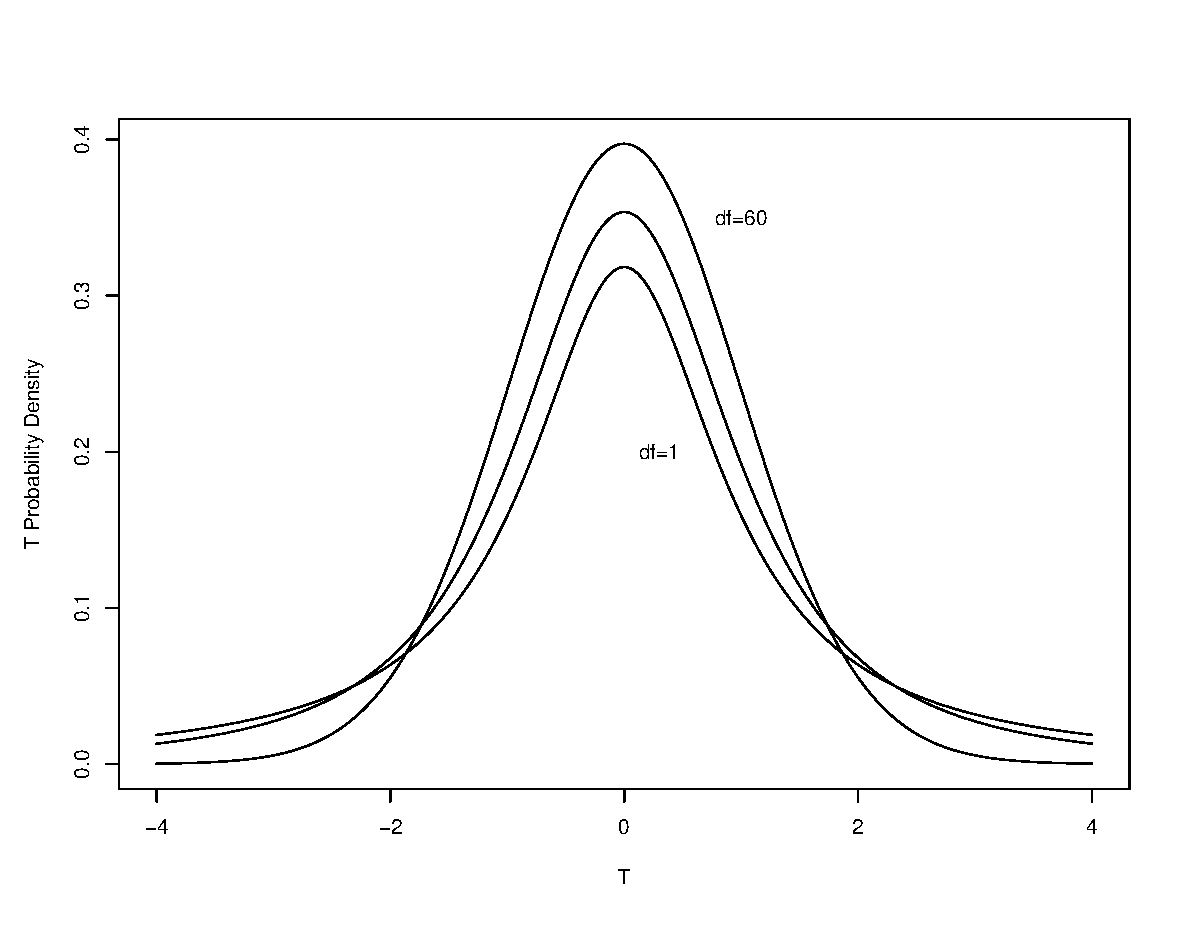
\includegraphics[width=5.5cm,height=3.5cm]{6tdistns}
\vskip-1cm
\end{center}
%> post()
%> plot(c(-400:400)/100, dt(c(-400:400)/100,
%> 1),type="l",ylim=c(0,dt(0,60)),xlab="T",ylab="T Probability Density")
%> lines(c(-400:400)/100,dt(c(-400:400)/100,60))
%> lines(c(-400:400)/100,dt(c(-400:400)/100,2))
%> text(.3,.2,labels="df=1")
%> text(1,.35,labels="df=60")
%> dev.off()
\vskip -0.6cm
\pause
{\bf Question:} What's the T distribution when $\nu \to \infty$?
\end{frame}
%%%%%%%%%%%%%%%%%%%%%%%%%%%%%%%%%%%%%%%%%%%%%%%

%%%%%%%%%%%%%%%%%%%%%%%%%%%%%%%%%%%%%%%%%%%%%%%
\begin{frame}{How is the $T-$distribution Related to Estimation?}
%%%%%%%%%%%%%%%%%%%%%%%%%%%%%%%%%%%%%%%%%%%%%%%

Let $X_1,X_2,\ldots,X_n$ be a random sample 
from a $N(\mu,\sigma^2)$ popn.
\medskip

We know that $\displaystyle Z=\frac{\bar{X}-\mu}{\sigma/\sqrt{n}}\sim N(0,1).$ \pause
\medskip

But what if $\sigma^2$ is not known? \pause
Use $s\approx\sigma$ to estimate it.
\bigskip

Consider
\begin{align*}
T &= \frac{\bar{X}-\mu}{s/\sqrt{n}} 
= \frac{\bar{X}-\mu}{\sigma/\sqrt{n}} \cdot \frac{\sigma}{s}
= Z \frac{\sigma}{s} \quad
 (\mbox{where\ } Z\sim N(0,1) )\\
&= \frac{Z}{s/\sigma} = \frac{Z}{\sqrt{s^2/\sigma^2}}\\
&= \frac{Z}{\sqrt{\frac{(n-1)s^2}{\sigma^2(n-1)}}}
 = \frac{Z}{\sqrt{\chi^2_{(n-1)}/(n-1)}}
\sim t_{(n-1)}
\end{align*}
\pause

\end{frame}
%%%%%%%%%%%%%%%%%%%%%%%%%%%%%%%%%%%%%%%%%%%%%%%

%%%%%%%%%%%%%%%%%%%%%%%%%%%%%%%%%%%%%%%%%%%%%%%
\begin{frame}{How is the $T-$distribution Related to Estimation?}
%%%%%%%%%%%%%%%%%%%%%%%%%%%%%%%%%%%%%%%%%%%%%%%

$T = \frac{\bar{X}-\mu}{s/\sqrt{n}} \sim t_{(n-1)}$ \pause

\bigskip

So, even when the popn variance $\sigma^2$ is not known, we can
still find probabilities for the sample mean $\bar{X}$ for data from a
normal popn. \pause  
\medskip

We just replace $\sigma$ by its estimate $(s)$ in the standardization of
$\bar{X}$ and then look up probabilities from the $t_{(n-1)}$ distribution
instead of the $N(0,1)$ distribution. \pause
\bigskip

The $t_{(n-1)}$ distribution is similar to the $N(0,1),$ but with more
spread (to account for the extra uncertainty in the estimate of $\sigma$.)
\medskip \pause

As sample size increases, $s$ gets closer to $\sigma$ \\
and the $t_{(n-1)}$ distribution gets closer to $N(0,1).$ \pause

\end{frame}
%%%%%%%%%%%%%%%%%%%%%%%%%%%%%%%%%%%%%%%%%%%%%%%






\end{document}
